\documentclass[12pt]{ctexrep}

\usepackage{graphicx}
\usepackage[hmargin=1.1in,vmargin=1in]{geometry}
\usepackage{indentfirst}
\usepackage{multirow}
\usepackage{makecell}
\usepackage{gbt7714}
\usepackage[defaultmono,scale=0.85]{droidsansmono}
\usepackage{minted}
\usepackage{color}
\usepackage[xetex,colorlinks=true]{hyperref}

\bibliographystyle{gbt7714-numerical}

\fontsize{14pt}{1.0}
\definecolor{codebg}{rgb}{0.95,0.95,0.95}

\newlength{\blanklength}
\setlength{\blanklength}{40ex}

\providecommand{\thetitle}{GNU GCC 项目设计逆向分析}
\providecommand{\theauthor}{Sparky\_14145}
\providecommand{\thestudentID}{71XXXXXX}
\providecommand{\theemail}{Sparky\_14145@outlook.com}
\providecommand{\theinstitution}{College of Software Engineering}

% \input{personal_info/info.tex}

\providecommand{\blankToFill}[1]{
    \parbox[t][3ex]{\blanklength}{
        \makebox[\blanklength]{#1}\\[0pt]
        \rule[2ex]{\blanklength}{0.1ex}
    }
}

\providecommand{\makecover}{\begin{titlepage}
    \noindent
    {东南大学} \\[2pt]
    {\Large \bfseries 实验报告}

    \vspace*{20pt}
    \begin{center}
    
\includegraphics[width=0.8\textwidth]{pics/cover.png} \\
        \textsc{\Huge 软件设计与体系结构课} \\[2pt]
        \textsc{\huge 实验报告}

        \vspace*{10pt}
        \begin{tabular}[c]{rc}
            题目        & \blankToFill{\thetitle} \\
            日期        & \blankToFill{\today} \\
            姓名        & \blankToFill{\theauthor\footnotemark} \\
            学号        & \blankToFill{\thestudentID} \\
            学院        & \blankToFill{\theinstitution} 
        \end{tabular}
        \rmfamily
    \end{center}

    \vspace*{0pt}
    % \begin{abstract}
    % \end{abstract}
    \footnotetext{\theemail}
\end{titlepage}}

\begin{document}
    \makecover

    \tableofcontents

    \chapter{课题概述}
    \section{选题简介}

    GNU 编译器套装(GCC)是一个流行的跨平台编译器套件,可以用于编译多种程序设计语言并生成可执行二进制文件。
    其支持的程序设计语言有:C, C++, Objective-C, Fortran, Ada, Go, D 以及汇编语言(AT \& T 语法),
    并为这些语言提供了一些库来方便用户进行开发。\cite{gcc-homepage}
    GCC 的目的是成为一个自由软件,从而为 GNU 项目提供支持。

    通过研究 GCC 的软件架构,我可以掌握一些关于编译器实现的知识,了解开源项目是如何设计与维护的;并且 GCC
    项目已有三十余年的历史,可以认为有大量的遗留代码甚至是遗留设计,通过研究该项目也可以学习到如何处理遗留
    代码等实用的软件项目管理技能。

    \section{实验的主要工作}

    开源项目 GCC 的逆向分析,主要包括:

    \begin{enumerate}
        \item 软件需求逆向分析;
        \item 软件架构逆向恢复;
        \item 软件架构分析评估。
    \end{enumerate}

    \chapter{需求逆向分析}
    \section{系统总体需求}

    本项目为 GNU 项目的一部分,目标是改进 GNU 系统(包括 GNU/Linux 变种)下编译器的使用体验。GCC 开发
    工作使用开放的开发环境,并支持许多其他平台,以产生一个世界级的优化编译器,吸引更大的开发团队,确保 GCC
    和 GNU 系统在多种架构和不同的环境中工作,并更彻底地测试和扩展GCC的功能。\cite{gcc-mission}

    本系统的总体用例图如下:

    \begin{figure}[h]
        \centering
        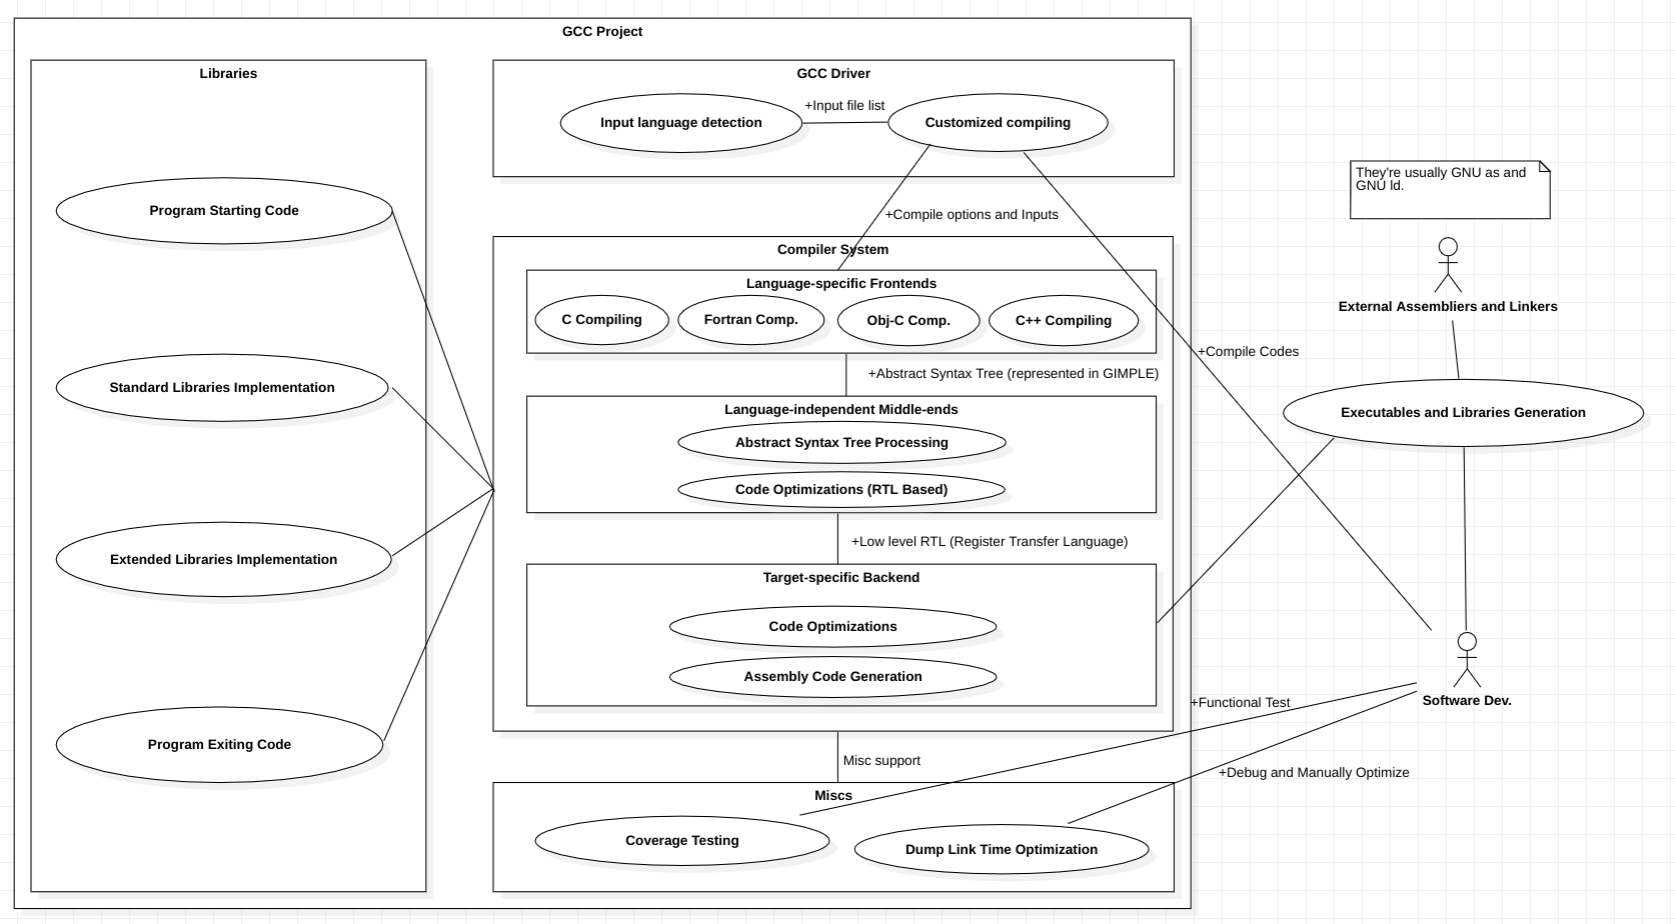
\includegraphics[width=0.8\textwidth]{pics/systemwide usecases.png}
        \caption{GCC 系统用例图}
    \end{figure}

    如图所示,GCC 主要分为六个模块:顶层的驱动(driver, 用于``一键''完成编译操作),语言相关的编译器
    前端(用来将各个语言的源码转换为语言无关的编译器内部使用的中间代码),语言无关的编译器中间层(用来
    将前端生成的中间代码转化为 RTL,并做一定程度的优化,从而方便后端生成汇编码),编译器后端(用来将中
    间层生成的非严格 RTL 转化为汇编代码)\cite{gcc-structure},
    一些杂项工具(提供诸如覆盖测试等的杂项功能),以及语言配套的编译、运行库等(包括标准库、启动代码以
    及一些扩展库)。其中,编译器驱动、前、中、后端四部分可以看成编译器系统的四个子模块,负责将给定的所有
    输入文件转化为汇编代码。

    用户在与 GCC 交互时,主要是与顶层的驱动,以及杂项工具相交互,而不与另外三个模块直接交互。向另外三个
    模块传递信息,以及调用外部汇编器、链接器等操作主要由顶层驱动负责完成。

    由于 GCC 项目与功能集规模过大,限于篇幅,本报告的剩余部分中无法涵盖 GCC 的全部内容,仅对部分主要与
    常用的用例等进行分析。

    \subsection{顶层驱动模块需求}

    在该模块,涉及的主要角色是用户(即其他程序的开发人员),以及外部的汇编器、链接器。

    模块的用例图如下(仅列举部分用例):

    \begin{figure}[hp]
        \centering
        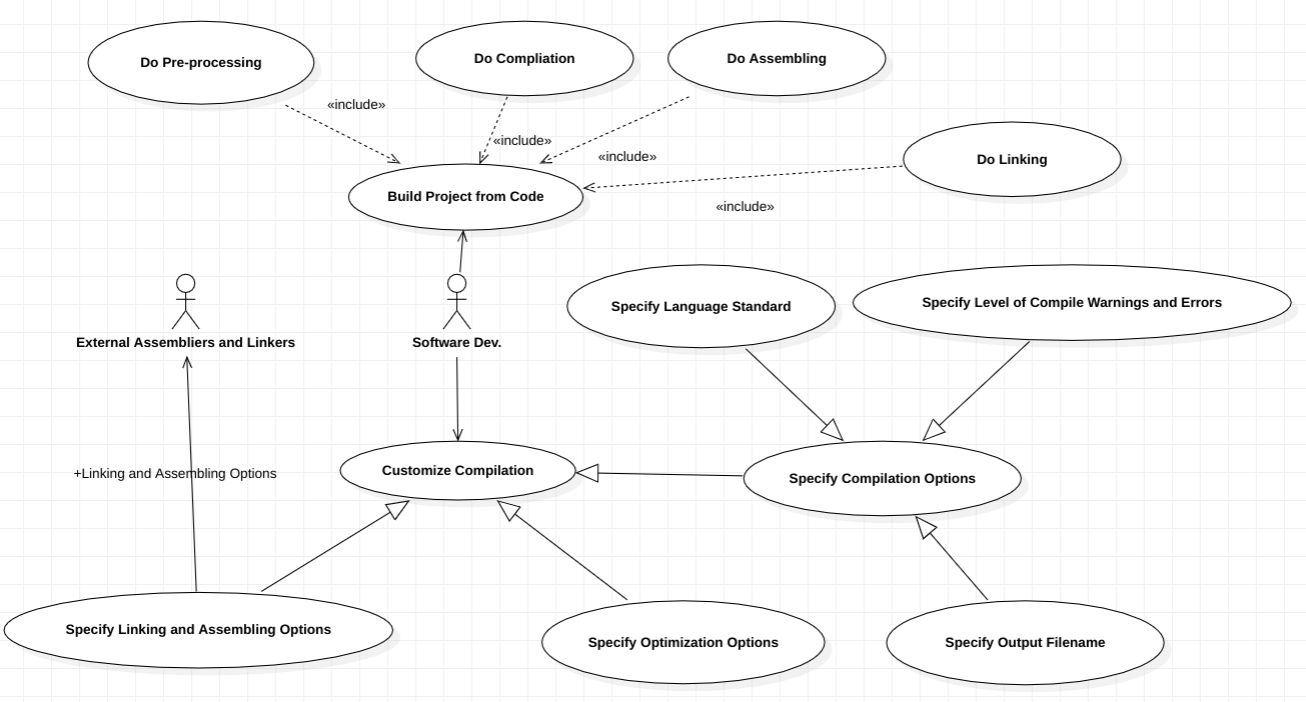
\includegraphics[width=0.8\textwidth]{pics/topentry usecases.png}
        \caption{顶层驱动用例图(部分)}
    \end{figure}

    顶层驱动模块主要负责与用户、外部程序的交互,以及协调 GCC 内部其他各个模块的工作。

    具体的用例说明如表 \ref{tab:topentry-usercases}。

    \begin{table}[hp]
        \centering
        \caption{顶层驱动用例说明表}
        \label{tab:topentry-usercases}
        \begin{tabular}{|c|c|c|}
            \hline
            角色 & 用例 & 功能 \\ \hline
            \multirow{11}{*}{用户(开发者)} & 客制化编译 & 按照需求定制编译过程。 \\ \cline{2-3}
             & 指定编译选项 & \makecell{修改编译器的部分行为,比如生成 \\ 文件名称、采用的语言标准(包括标准版本 \\ 以及是扩展标准还是 ISO 标准)、如何生成 \\ 错误信息、如何处理警告等等。} \\ \cline{2-3}
             & 指定优化开关 & \makecell{修改编译器的优化行为,比如以减 \\ 小代码体积为目标还是以加快执行速度为 \\ 首要目标,或者是一些更加细节的优化行为。} \\ \cline{2-3}
             & 指定汇编链接选项 & \makecell{令 GCC 在调用外部汇编、链接器的 \\ 时候传递某些参数,从而改变 \\ 外部汇编、链接器的某些行为} \\ \hline
            \multirow{1}{*}{编译器} & 构建项目 & \makecell{按照用户的客制化需求生成指定内容 \\(二进制代码等)。} \\ \hline
        \end{tabular}
    \end{table}

    \subsection{编译器系统其他模块需求}

    编译器系统模块主要负责将驱动模块指定的文件转化为平台上的汇编代码,可以分为三个子模块:前端,中间层和后端。

    编译器前端模块主要负责将源码转化为 GIMPLE\cite{gineric-and-gimple} 表示的树形中间代码\cite{gcc-frontend}。

    编译器中间层主要负责将前端传来的 GIMPLE 表示的中间代码转化成非严格 RTL\cite{gcc-rtl} 代码供后端生成汇编码\cite{gcc-structure}。

    编译器后端主要负责将中间层传来的非严格 RTL 代码转化为严格 RTL 代码,进一步优化,以及最终生成汇编码\cite{gcc-backend}。

    \subsection{运行库模块需求}

    运行库模块主要负责提供各个语言的运行时的启动代码、退出代码,编译时语言标准库的实现以及扩展库的实现。具体
    说明见表 \ref{tab:runtime-lib-usercases}。

    \begin{table}[hp]
        \centering
        \caption{运行库模块用例说明表}
        \label{tab:runtime-lib-usercases}
        \begin{tabular}{|c|c|c|}
            \hline
            角色 & 用例 & 功能 \\ \hline
            用户 & 库实现参考 & \makecell{利用标准库和扩展库的实现或声明 \\ 编写代码或者改进已有实现。} \\ \hline
            编译器 & 库实现参考 & \makecell{检查用户代码对标准库与扩展库的 \\ 引用是否正确,并生成警告或错误。} \\ \hline
            外部汇编器 & 启动(退出)代码参考 & \makecell{为外部汇编器提供平台特定的 \\ 启动(结束)代码,让链接器 \\ 能够生成正常运行、结束的二进制文件。} \\ \hline
        \end{tabular}
    \end{table}

    \subsection{杂项模块需求}

    此模块提供一些杂项功能,诸如覆盖测试、导出链接时优化等功能,以及一些供编译器系统模块使用的、原本不属于
    GCC 项目的一些功能(比如 \verb|nm|,\verb|ar| 等属于 GNU Binutils 项目的工具)。

    \section{本章小结}

    本章主要介绍了系统的需求分析,包括系统功能性需求,并通过使用用例图介绍了四个模块的具体功能,通过表格详细
    分析了用例图。

    \chapter{软件架构逆向恢复}
    \section{系统的总体架构}

    本项目的总体架构为仓库风格:运行库模块和用户提供的程序源码(或二进制文件等)共同组成了系统的数据,然后
    其他各个模块围绕这些数据履行各自的职责(代码转化等等)。

    本项目高度可客制化,在构建本项目时,用户可以根据需要自由定义调用外部链接器、汇编器时的路径、系统生成的
    代码的目标平台、系统构建项目时使用的线程模型,以及需要支持的语言集等等。\cite{gcc-configure}

    本项目的各个内部模块需要在编译时确定,即本项目不提供在构建完成后额外引入/卸载模块的方法(运行库模块除
    外)。如果需要额外引入模块(如添加对其他语言的支持),需要修改项目源码并重新编译本项目。

    \section{各组件的设计}
    \subsection{编译器系统组件的设计}

    该组件为 GCC 项目的核心组件,负责将给定的文件转化为汇编码、并可能将之进行汇编、链接。该组件内部采用的
    软件架构风格为黑板风格,其中,编译器顶层驱动为黑板的控制器,根据不同的输入文件确定如何安排其他各个编译
    子模块工作,并收集它们工作时产生的信息。

    \subsubsection{编译器顶层驱动组件的设计}

    该组件为编译器系统的控制组件,负责与用户交互,为其他组件``分配任务'',并收集其他组件产生的信息,为其他
    组件分配、回收临时文件等工作。可以认为这个组件是整个编译器系统的``包装器''。

    该组件内部架构风格为批处理风格:对于每一次运行,该组件均会按照顺序,执行以下操作:

    \begin{enumerate}
        \item 设置程序名称(用于显示帮助信息);
        \item 解析命令行参数(确定输入文件列表、确定客制化编译选项等);
        \item 进行全局初始化,建立 \verb|SPEC| 列表(\verb|SPEC| 用来描述对输入文件应当执行的操作);
        \item 处理环境变量;
        \item 处理未知选项;
        \item 准备输入文件(确定对每个输入文件需要做什么);
        \item 对每个输入文件,利用 \verb|SPEC| 机制对其进行处理;
        \item 运行外部链接器;
        \item 删除残余的临时文件。
    \end{enumerate}

    如以下代码所示:

    \begin{minted}[bgcolor=codebg,autogobble,linenos=true,breaklines]{cpp}
/* driver::main is implemented as a series of driver:: method calls.  */
        
int
driver::main (int argc, char **argv)
{
  bool early_exit;

  set_progname (argv[0]);
  expand_at_files (&argc, &argv);
  decode_argv (argc, const_cast <const char **> (argv));
  global_initializations ();
  build_multilib_strings ();
  set_up_specs ();
  putenv_COLLECT_AS_OPTIONS (assembler_options);
  putenv_COLLECT_GCC (argv[0]);
  maybe_putenv_COLLECT_LTO_WRAPPER ();
  maybe_putenv_OFFLOAD_TARGETS ();
  handle_unrecognized_options ();

  if (completion)
    {
      m_option_proposer.suggest_completion (completion);
      return 0;
    }

  if (!maybe_print_and_exit ())
    return 0;

  early_exit = prepare_infiles ();
  if (early_exit)
    return get_exit_code ();

  do_spec_on_infiles ();
  maybe_run_linker (argv[0]);
  final_actions ();
  return get_exit_code ();
}
    \end{minted}

    其中 \mintinline{cpp}{final_actions()} 函数负责进行删除临时文件等工作。

    项目的其他组件一般不会直接调用编译器驱动组件,而是被该组件调用。

    GCC 的官方源码编译出的二进制文件中,可能包含以下编译器驱动(可随编译时的配置而改变):

    \begin{itemize}
        \item \verb|gcc|(通常用于编译 \verb|C|,但也可以编译 \verb|C++| 等);
        \item \verb|g++|(通常用于编译 \verb|C++|,但也可以编译 \verb|C| 等);
        \item \verb|gfortran|(用于编译 \verb|fortran|);
        \item \verb|gdc|(用于编译 \verb|D|)。
    \end{itemize}

    \subsubsection{编译器前端组件的设计}

    编译器前端模块主要负责将源码转化为中间代码。根据各个前端的实现不同,编译器前端可能会将源码转换为
    \verb|GENERIC|,\verb|GIMPLE|,或者是其他的表示形式。\cite{gcc-parsing-pass}

    编译器前端采用了批处理的架构风格:在将源码转化为中间代码时,编译器前端会按照编译器开发人员给定的
    顺序,依次对源码执行一些操作(或者是调用其他的组件(passes))来对代码进行变形等操作。

    编译器前端往往和后端及中间件打包在一起,成为一个可执行文件,并且如一般的命令行可执行文件那般接收
    命令行参数供调用。

    GCC 的官方源码编译出的二进制文件中,可能包含以下前后端打包在一起形成的可执行文件:

    \begin{itemize}
        \item \verb|cc1|,用于编译 \verb|C|;
        \item \verb|cc1plus|,用于编译 \verb|C++|;
        \item \verb|cc1obj|,用于编译 \verb|Objective-C|;
        \item \verb|cc1objplus|,用于编译 \verb|Objective-C++|;
        \item \verb|f951|,用于编译 \verb|Fortran|;
        \item \verb|d21|,用于编译 \verb|D|。
    \end{itemize}

    \subsubsection{编译器中间层组件的设计}

    编译器中间层组件实际上由一个组件管理器(Pass Manager)和众多其他组件集合而成的\cite{gcc-pass-manager}。
    整个中间层组件采用了插件-平台风格,供前后端进行调用。

    组件管理器(定义于头文件 \verb|gcc/pass_manager.h|)提供了注册组件、获取组件、导出组件、批量执行
    组件等接口方法,且组件可以按照名称或 ID 进行索引。每个组件要求为以下类型之一(由于 C++ 本身没有较为
    完善的反射机制,这些类型由实例的内部枚举字段 \verb|type| 进行标识):

    \begin{minted}[autogobble,linenos=true,bgcolor=codebg,breaklines]{cpp}
/* In file gcc/tree-pass.h, line 31 */
enum opt_pass_type
{
  GIMPLE_PASS,
  RTL_PASS,
  SIMPLE_IPA_PASS,
  IPA_PASS
};
    \end{minted}

    而各个组件的注册方法,其一是在 \verb|gcc/passes.def| 中声明相关内容(然后,极其硬核地,通过宏展开的
    方式在编译时注入到源码中,成为 \verb|pass_manager| 类的一个指针成员);其二是运行时通过 \verb|pass_manager|
    类的相关接口进行注册。

    \subsubsection{编译器后端组件的设计}

    编译器后端组件主要负责将中间代码转化为目标平台上的汇编代码。

    在上文中提到的``前端和后端打包在一起生成的可执行文件''中,每一个可执行文件实际上只会包含一个平台的
    一个后端,具体是哪一个取决于编译时给定的配置\cite{gcc-configure}(配置构建时使用选项
    \verb|--target=<TARGET>| 指定)。

    \subsection{运行库模块设计}

    运行库模块,如需求分析中所述,负责提供各种编译期、链接期的实现参考,以及启动代码、终止代码的实现。

    由于本身不需要被执行,该模块实质上只是许多文件的集合,另外提供了一些方便模块自身维护的测试工具,以及
    一些为了在构建编译器系统时能够正确给不同平台提供参考而存放的构建脚本等内容。

    该模块没有刻意提供某些接口——该模块存在的意义就是供其他模块参考,因此本模块中,所有非实现细节内容对
    其他模块均可见。

    \subsection{杂项模块设计}

    杂项模块负责提供一些杂项功能,从功能角度而言并非整个 ``GCC 编译器'' 的一部分。

    这个模块由一些彼此独立的子模块组成,已知的模块如下:

    \begin{itemize}
        \item \verb|gcov|,代码覆盖测试工具\cite{gcc-gcov},拥有两个辅助工具:
        \begin{itemize}
            \item \verb|gcov-tool|;
            \item \verb|gcov-dump|。
        \end{itemize}
        \item \verb|lto-dump|,导出链接时优化目标文件(link time optimization object files)\cite{gcc-lto-dump};
        \item \verb|gcc-ar|,归档工具,与 GNU ar 的区别是会自动传递 LTO 插件(Wrapper to \verb|ar| to pass the LTO plugin),下同。拥有一个变种:
        \begin{itemize}
            \item \verb|gcc-ranlib|,等同于 \verb|gcc-ar -s|。
        \end{itemize}
        \item \verb|gcc-nm|,从目标代码中导出符号。
    \end{itemize}

    \section{连接件设计}

    \subsection{驱动与前端的连接件设计}
    \label{subsec:conn-1}

    驱动与前端(或者严格来说时驱动与前、后端的可执行文件)采用了主/子程序的风格来连接。编译器驱动通过一种叫
    做 \verb|SPEC| 的机制调用 \verb|liberty| 库中的 \verb|pex_run| 等函数来令编译器前端编译文件。
    而这些函数(在 Linux 系统上)最终会通过 \verb|execvp| 等系统调用来执行可执行文件。

    \subsection{前端与中间件、后端的连接件设计}

    前端与后端的连接在构建编译器时建立。一个可执行文件中只会包含一个前端与一个后端,而最终整个编译器在
    一次构建完成后会生成数量等同于编译前配置时给定的前端数目的此类可执行文件(一次构建只能指定生成一个
    后端)。并且,所有的中间件也会被打包进每一个此类可执行文件(包括中间件管理器)。
    
    前后端在调用中间件时,直接在自身线程内调用目标中间件对象的 \verb|execute| 方法,或者(也是在自身
    线程内)调用管理器对象的某些方法,令其在自身线程内执行。

    \subsection{与外部链接器、汇编器的连接件}

    同 \ref{subsec:conn-1}。

    \section{本章小结}

    本章主要介绍了该系统的设计。首先从总体出发,描述的系统的总体模块,然后从六大模块详细分析各个模块的内
    容。在最后,介绍来各个模块之间的连接方式。

    \chapter{软件架构分析}

    整个编译器项目采用了仓库风格的软件架构,将用户的源码(包括第三方库)与运行库作为仓库数据,供系统中
    (除运行库以外的)各个组件处理。

    采用仓库风格的好处有:

    \begin{enumerate}
        \item 编译器天然便是以数据(源码)为中心的系统,很适合使用仓库风格;
        \item 将运行库也作为仓库中的数据,便于用户客制化编译(比如,使用第三方库,甚至是禁止使用标准库(Linux 内核/内核模块))。
    \end{enumerate}

    而在连接各个模块的时候,可以看到系统要么使用了``静态链接''(将相关的模块打包在一起),要么使用了主/子
    程序的方法。这么做的好处有:

    \begin{enumerate}
        \item 提高了系统运行时的效率。由于不需要复杂的子系统去维护模块连接,系统的运行效率得到了提高。
    \end{enumerate}

    而缺陷也很明显:

    \begin{enumerate}
        \item 对于构建完成的系统,客制化能力降低。由于大量采用``静态链接'',在编译器系统构建完成以后,如果想要新增前、后端,只能修改配置,重新构建;
        \item 构建系统时,所有东西必须均可见。这也就导致了整个项目的源码``臃肿不堪''(一个代码仓库同时维护了编译器驱动、前后端、中间件以及众多语言的运行库,整个仓库大小高达 1GB,且一次构建需要至少四小时);
        \item 主/子程序的方法来调用其他组件,要么难以利用现代计算机系统的多线程能力,要么需要手动处理多线程的情况。
    \end{enumerate}

    \chapter{实验小结}

    本次实验通过阅读 GNU GCC 项目的源码、文档,对项目进行了软件需求、设计、架构等的逆向分析,让我得到了以下经验:

    \begin{enumerate}
        \item 仓库风格很适合用于编译器的整体项目设计;
        \item 珍爱生命,远离 \verb|Makefile|,特别是那种一个项目好几个上万行的 \verb|Makefile| 甚至混合 \verb|autoconf| 的项目,单凭阅读源码很难了解整个项目的结构;
        \item 不要因为 C++ 兼容 C,就理所应当地在同一个文件混用两种语言。应该没有谁会喜欢那种同一个文件里同时看到 \mintinline{cpp}{int driver::main(int argc, char* argv[])} 和 \mintinline{cpp}{void func(void)} 这两种声明的感觉吧;
        \item 对于年代比较久远的项目,适时重构是很重要的一件事情。比如对于本项目,始于上世纪八十年代,当时应该有很多项目风格、软件工程理论没有被提出,也就导致了本项目一开始(相对如今的许多项目)``比较落后'',而长时间没有重构更是使得落后的项目风格问题愈发明显,也让项目变得更加的难以维护;
        \item 养成写文档和注释的良好习惯。虽然本项目的整体偏落后,但文档和注释却很详尽(对于概览来说。具体实现上仍然有大量文档缺失),这使得我能够在短时间内理解项目结构;也是因为文档缺失,在很多实现细节上我仍然没有弄清楚。
    \end{enumerate}

    \bibliography{citations}
\end{document}